% Created:  Fri 01 Aug 2014 02:02 PM
% Modified: Wed 06 Aug 2014 10:26 am
% @author Josh Wainwright
% filename: analysis.tex

\section{Cluster Analysis}
\label{sec:cluster_analysis}

Once the data has been processed and a number of clusters have been identified,
they can be displayed on screen in an image to verify what was found and
perform further analysis. However, since the data that was used to find the
clusteres is still held in memory at this point, it is useful to take advantage
of this and perform some imediate analysis and provide some statistics
regarding the clusters that were found.

There are two ways of conceptually viewing the clusters which will lead to
slightly different results when analysing them.

\begin{itemize}

	\item The first is to consider the boundary of the nodes of the quadtree
		that were considered to be part of a cluster to be the boundary of the
		cluster. This will mean that the actual cluster is likely to be
		slightly larger than the actual data points that it is comprised of,
		but is computationally simple to acheive, so fast, and can take into
		account any holes in the cluster.

	\item The second way is to, once the cluster has been located, disgard the
		information about the nodes themselves, and simply use them to select
		the appropriate points. This results in a set of points that are all
		considered to be spatially grouped into the same cluster. From this
		set, calculations can be performed on the real data. This method is
		garanteed to provide information that more closely represents the
		original data, though is more computationally intensive.

\end{itemize}

\subsection{Quadtree Node Analysis}
\label{sub:quadtree_node_analysis}

Here, the nodes of the quadtree that were considered part of the cluster are
considered, rather than the points that they contain.

\subsubsection{Cluster Area}
\label{ssub:Cluster Area}

To calculate the area of the clusters, each node in each cluster is examined.
Since the size of the node must be known, it is calculated from the quadtree
code for that node. The formula is shown in Equation~\ref{eq:node-area},
\begin{align}
	a &= \frac{1}{4^{d}} \\
	a_i &= 4^{-l_i/2}, \label{eq:node-area}
\end{align}
where $a_i$ is the area of the node $i$, $d$ is the depth in the quadtree and
$l_i$ is the length of the quadtree code of that node. For every node in the
cluster, where there are $n$ nodes, this value is summed to give the total
cluster area, $A$:
\begin{align}
	A &= \sum_{i=0}^{n} a_i.
\end{align}

\subsubsection{Cluster Perimeter}
\label{ssub:Cluster Perimeter}

Similarly to the cluster area, the perimeter is given as a fractional value of
the length of one side of the whole image, as calculated for each node from the
quadtree code, as shown in Equation~\ref{eq:node-perimeter},
\begin{align}
	p &= \frac{1}{2^{d}} \\
	p_i &= 2^{-l_i/2}, \label{eq:node-perimeter}
\end{align}
where the symbols have the same meaning as above.

However, this simply gives the length of one side of the node for any node. In
order to calculate the perimeter of the cluster, it is not enough to simply
sum these values, as for the cluster area, since not all nodes contribute to
the perimeter. Instead, for each node, it must be decided whether it
contributes to the perimeter and how much (1, 2, 3 or 4 sides), and then
increase the total perimeter by this many times the length of one side. The
total perimeter, $P$, then is given by Equation~\ref{eq:total-perimeter},
\begin{align}
	P &= \sum_{i=0}^{n} s * p_i, \label{eq:total-perimeter}
\end{align}
where $s \in \{0..4\}$. This is demonstrated in
Figure~\ref{fig:perimeter-edges} where the perimeter is simple to calculate in
case a) as the nodes are all the same, but the size of each node must be taken
into account in case b).

\begin{figure}[tbhp]
	\centering
	\begin{subfigure}[c]{3.5cm}
		\includegraphics[width=\textwidth]{perimeter-edges-grid.pdf}
		\caption{}\label{fig:perimeter-edges-grid.pdf}
	\end{subfigure}%
	\quad
	\begin{subfigure}[c]{3.5cm}
		\includegraphics[width=\textwidth]{perimeter-edges-quadtree.pdf}
		\caption{}\label{fig:perimeter-edges-quadtree.pdf}
	\end{subfigure}

	\caption{When calculating the perimeter of a cluster using the nodes that
		contribute, the size of each node must be taken into account. In
		case~\subref{fig:perimeter-edges-grid.pdf}, the process is simple since
		all nodes are the same size and a fractional value of 3.5 is
		calculated. For case~\subref{fig:perimeter-edges-quadtree.pdf}, the
		steps are 25 lengths of size $\rfrac{1}{8}$ and 6 lengths of size
		$\rfrac{1}{16}$ which gives the same result, 3.5.}
	\label{fig:perimeter-edges}

\end{figure}

Within the cluster, \emph{holes} occur where a node, or number of nodes, is
surrounded on all sides by the same cluster. An example can be seen in
Figure~\ref{fig:kernel-options}. Unfortunately, these are included in the
calculation of the perimeter and so, where holes exist in a cluster, the actual
perimeter is slightly smaller than that calculated.

\subsubsection{Cluster Roundness}
\label{ssub:Cluster Roundness}

A potentially useful measure of a cluster is its \emph{roundness}. This
describes the extent to which the area and perimeter of the cluster resemble a
circle. The avialible values of roundness are from 0, meaning a perfect line
with no area but finite perimeter, to 1, being a perfect circle. The equation
to determine roundness, Equation~\ref{eq:roundness} is defined such that it is
a unitless ratio of area and perimeter, such that a circle has roundness 1. The
derivation of Equation~\ref{eq:roundness} is found in
Appendix~\ref{app:roundness_derivation}.

\begin{align}
	R &= \sqrt{\frac{4\pi A}{p^2}} \label{eq:roundness}
\end{align}

The clusters that are found for data sets \texttt{palm-1.txt} and
\texttt{palm-2.txt} are shown in Figure~\ref{fig:roundness}. The roundness
values for the clusters for these data are very different,
Figure~\ref{fig:roundness-long.png} has an average $R=0.350$ whereas
Figure~\ref{fig:roundness-round.png} has an average $R=0.446$.

\begin{figure}[tbhp]
	\centering
	\begin{subfigure}[b]{4.2cm}
		\fbox{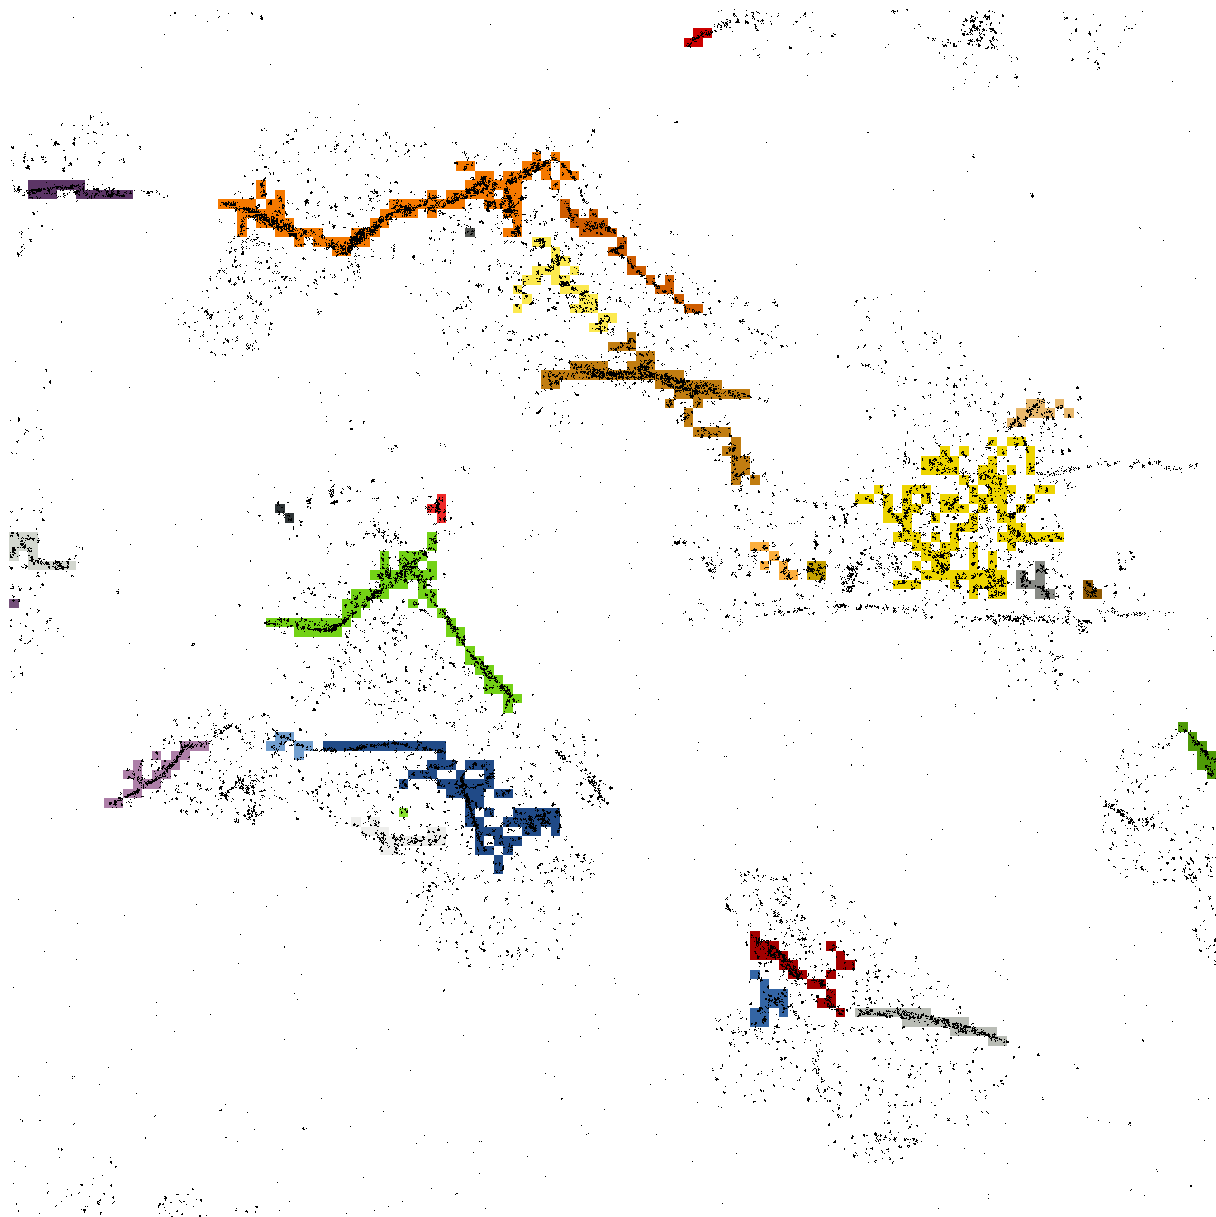
\includegraphics[width=\textwidth]{roundness-long.png}}
		\caption{}\label{fig:roundness-long.png}
	\end{subfigure}%
	\quad
	\begin{subfigure}[b]{4.2cm}
		\fbox{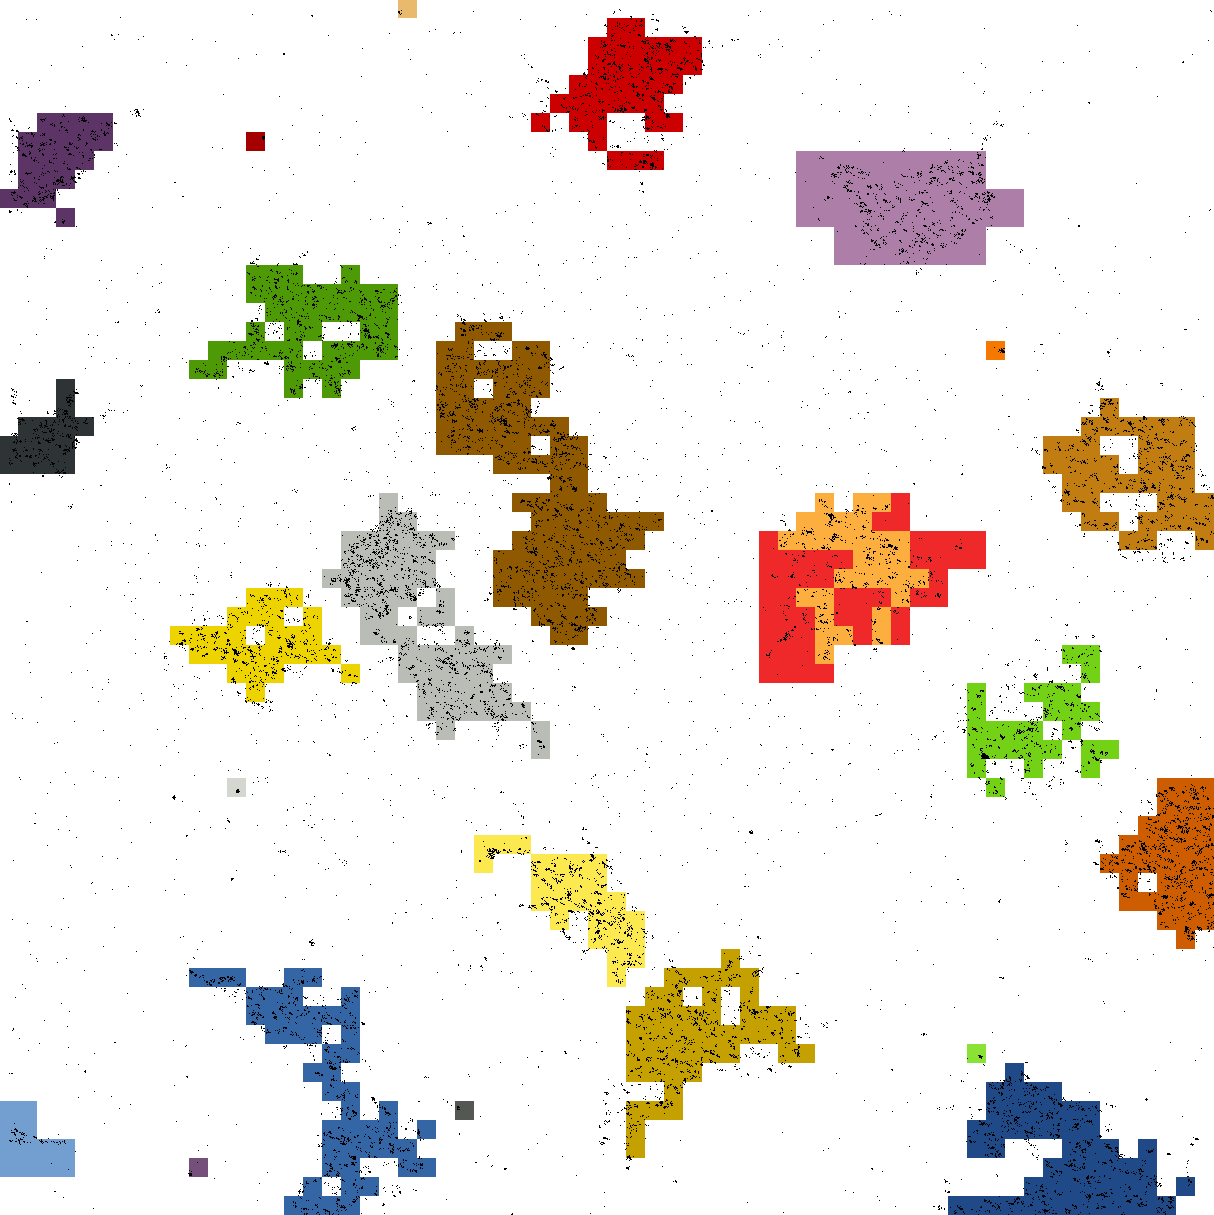
\includegraphics[width=\textwidth]{roundness-round.png}}
		\caption{}\label{fig:roundness-round.png}
	\end{subfigure}
	\caption{The general shape of the clusters found can be described using the
		roundness measure. A value closer to 0 means longer and thinner
		clusters, whereas values closer to 1 mean clusters that are more
		circular.} \label{fig:roundness}
\end{figure}

\subsection{Point Analysis}
\label{sub:point_analysis}

Here, the points contained in the nodes of quadtree that were considered part
of the cluster are considered; the nodes are only used to select the correct
points.

\subsubsection{Cluster Area}
\label{ssub:Cluster Area}

% TODO cluster area with points

\subsubsection{Cluster Perimeter}
\label{ssub:Cluster Perimeter}

% TODO cluster perimeter with points

\cite{lee2002polygonization}

\cite{estivill2000autoclust}

\cite{xia2006border}
